\documentclass[a4paper]{article}

\usepackage[catalan]{babel} % Language 
\usepackage{fontspec}
\usepackage[margin=2cm]{geometry}
\usepackage{float}
\usepackage{pgfplots}
\usepackage{pgfplotstable}
\usepackage[hidelinks]{hyperref}
\usepackage{enumitem}
\usepackage{amsmath}
\usepackage{gensymb} % For the degree symbol
\usepackage{graphicx}
\usepackage{longtable}

\setlength{\parindent}{0pt}
\setlength{\parskip}{1em}

\title{Projecte APA}
\author{Joan Marcè \and Esteve Tarragó}

\begin{document}
\maketitle
\tableofcontents
\newpage

\section{Introducció}

En aquest treball s'ha de realitzar una aplicació pràctica dels diferents coneixements de \emph{Machine Learning} adquirits a classe. Així doncs, s'ha escollit un conjunt de dades per realitzar una aplicació pràctica mitjançant mètodes de classificació. 

El conjunt de dades escollit ha estat \emph{Grammatical Facial Expressions Data Set}. Aquests han estat obtinguts mitjançant una càmera \emph{Kinect} que ha enregistrat diferents punts (100) en tres dimensions de la cara de diverses persones al llarg del temps mentre realitzen una paraula en el llenguatge de signes brasiler. Aquestes expressions van combinades amb gestos amb la mà però en aquest cas només s'ha gravat la cara. Després, aquests conjunts han estat analitzats manualment per decidir quins fotogrames estan fent realment una expressió facial i quins no. 

Les dades es poden obtenir en el següent enllaç:  \url{http://archive.ics.uci.edu/ml/datasets/Grammatical+Facial+Expressions}

A part, aquestes dades també s'han usat en treballs anteriors \cite{freitas}.

\begin{figure}[H]
	\centering
	\fbox{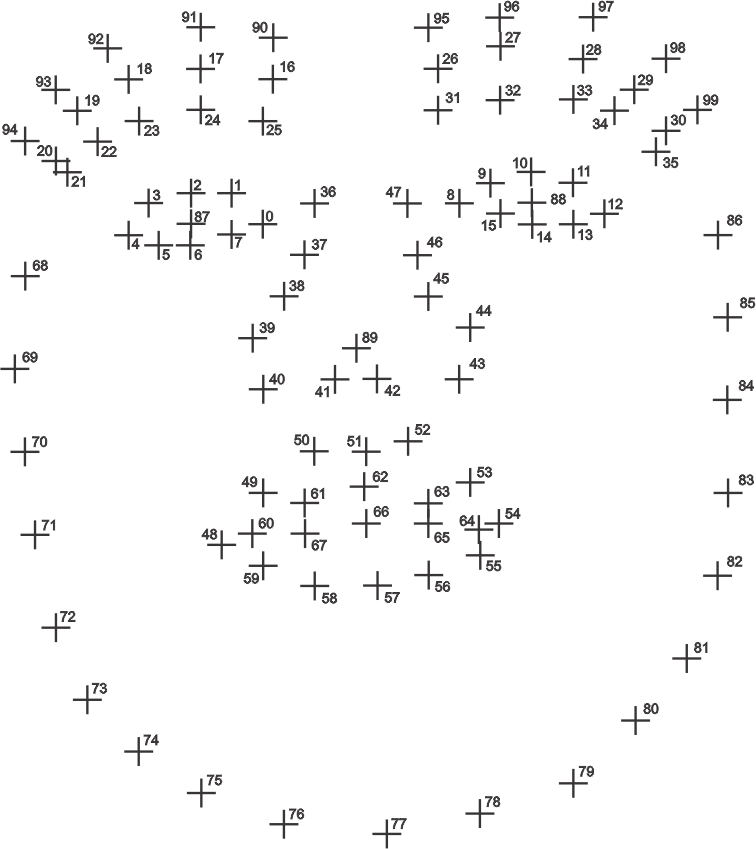
\includegraphics[width=0.6\textwidth]{images/view_points}}
	\caption{Representació dels punts de la cara que són utilitzats en la presa de dades}
\end{figure}

\section{Objectius}

L'objectiu d'aquest treball és poder decidir a partir d'una dada no usada prèviament:
\begin{enumerate}
	\item A partir d'una sola expressió facial si aquella s'està realitzant o no.
	\item A partir de tot el conjunt de dades si s'està realitzant o no una expressió facial.
	\item En el cas en el que s'estigui realitzant una expressió facial, poder decidir de quin tipus d'expressió facial (o paraula) es tracta.
	\item Trobar quin tipus de model s'adequa millor als objectius anteriors i comprar-los entre ells.
\end{enumerate}

\section{Procés d'exploració de dades}

S'han realitzat dos \emph{scripts} en R. El primer és per visualitzar les dades cronològicament (\verb|loadData.R|) i el segon és per poder interpretar-les a l'hora de realitzar una classificació (\verb|clustering.R|).

En aquest cas interessa més el segon ja que és el que tracta el problema de \emph{clustering}. S'han realitzat dos tipus d'algoritmes\cite{bishop} per projectar les dades, FDA i PCA. L'\emph{script} requereix que es seleccioni primerament quina expressió (\verb|*_datapoints.txt|) i a continuació quins resultats (\verb|*_targets.txt|) es volen agafar. També cal introduir de quin punt es volen visualitzar les dades (variable \verb|point|). 

A continuació es mostren els resultats obtinguts amb el conjunt de dades \verb|a_affirmative_datapoints.txt| i \verb|a_affirmative_targets.txt| i el punt 60 que correspon a la part superior del llavi. Per representar les dades s'han restat les mitjanes per tal que tant els punts com la recta de projecció estiguin centrades al voltant de $(0,0)$.

\begin{longtable}{cc}
	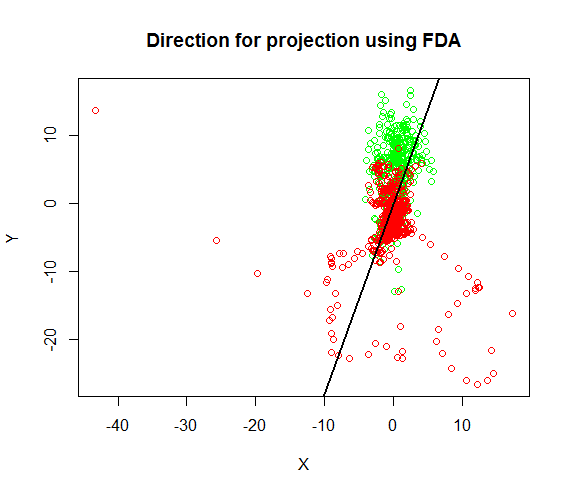
\includegraphics[width=0.45\textwidth]{images/FDA_XY} &
	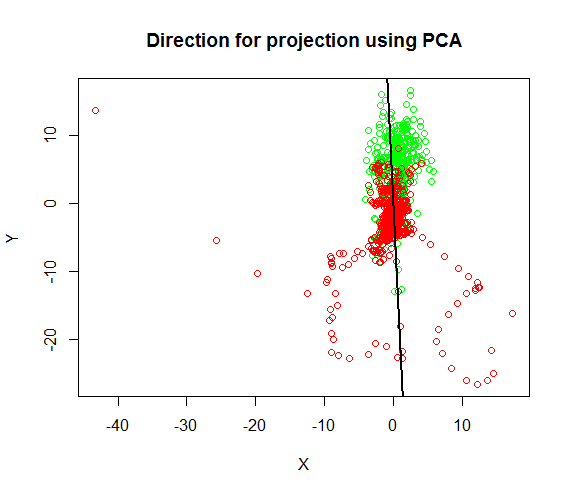
\includegraphics[width=0.45\textwidth]{images/PCA_XY} \\
	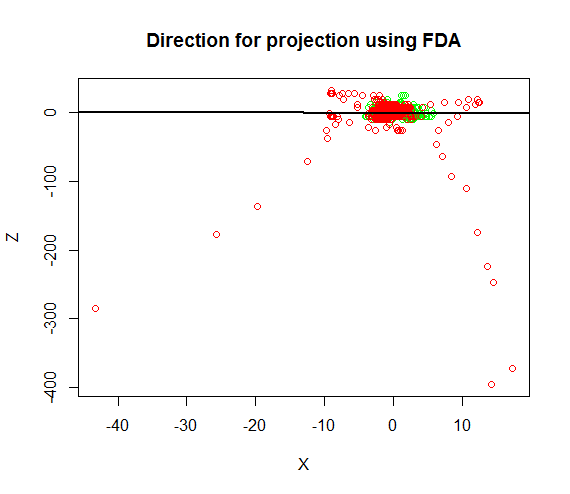
\includegraphics[width=0.45\textwidth]{images/FDA_XZ} &
	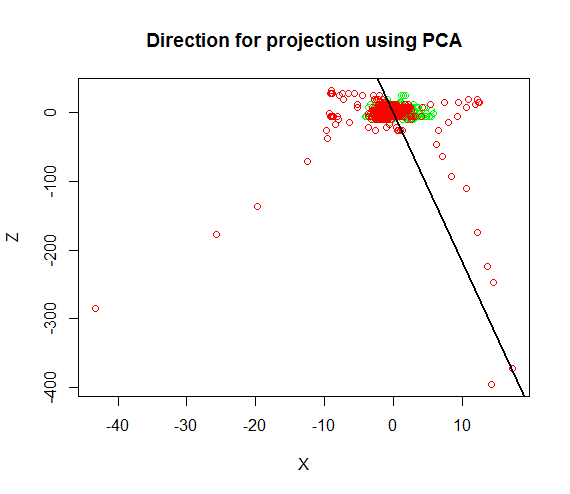
\includegraphics[width=0.45\textwidth]{images/PCA_XZ} \\
	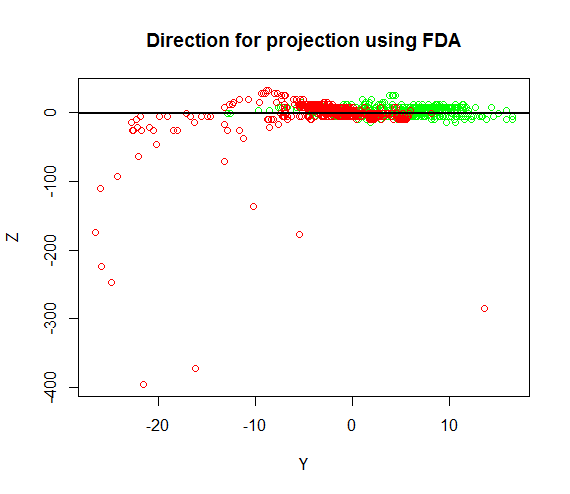
\includegraphics[width=0.45\textwidth]{images/FDA_YZ} &
	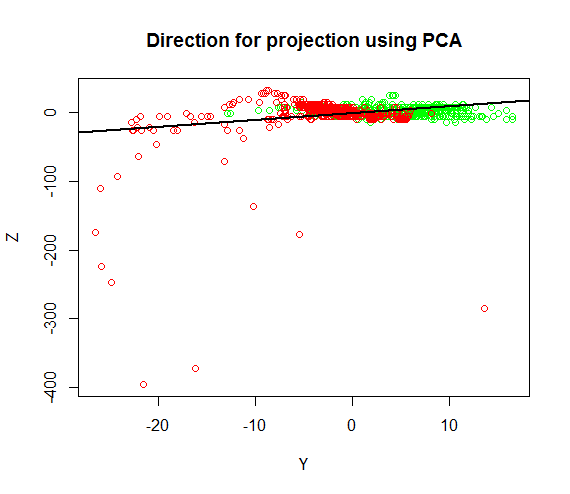
\includegraphics[width=0.45\textwidth]{images/PCA_YZ} \\
	\multicolumn{2}{c}{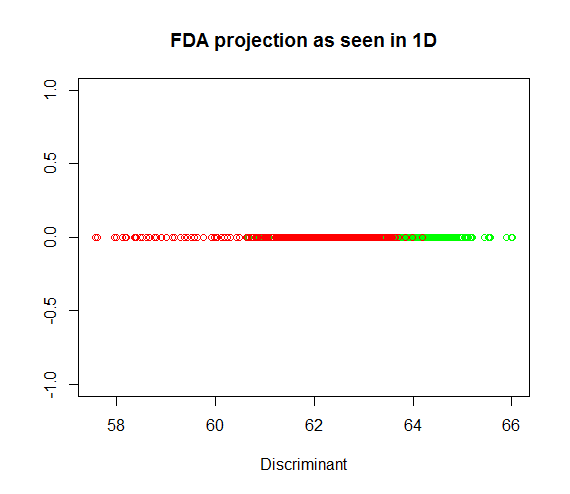
\includegraphics[width=0.5\textwidth]{images/FDA_projection}}
\end{longtable}

Com es pot veure als gràfics anteriors la dada Z no permet agrupar les dades gaire bé ja que totes queden al voltant dels valors \verb|Z = 0|. 

\section{Resultats amb mètodes lineals/quadràtics}
\section{Resultats amb mètodes no lineals}
\section{Model final escollit}
\section{Conclusions}
\section{Possibles extensions}
\section{Referències}

\bibliographystyle{acm}
\bibliography{bibliography}

\end{document}